% !TeX root = ../main.tex
% Add the above to each chapter to make compiling the PDF easier in some 


\chapter{Experimental Setup}\label{chapter:experimental_setup}


In this section, we will explain different types of experimental environments, reward, and observation structures.  


\section{Problem Setup}

We base our environment setting on Breyer et al.'s table cleaning grasping environment. In the simulation environment, a gripper is spawned until the wrist and attempts to grasp randomly drawn objects from the table or the floor. The gripper is deprived of an arm and a base. Accordingly, the computation of inverse kinematics is ignored.

The observed state originates from the RGBD camera mounted on the gripper. The gripper is position controlled with continuous input between -1 to 1. Based on the task description, an action is represented either by [dx, dy, dz, \(\phi\), gripper open/close] or [dx, dy, \(\phi\)]. 

Episode either terminates by the timeout signal after 150 timesteps or the success signal. Success signal is triggered when the gripper carries an object to a predefined height defined by the curriculum strategy.

We conduct our experiments on two different simulation scenes: Floor (\ref{fig:table}) and table with a tray (\ref{fig:floor}). Floor scene represents the Breyer et al.'s setup, and the table with a tray scene is same as the Quillen et al.'s configuration. We investigated the transfer performance of the model trained in the floor scene in the table setup.

Different task descriptions will be explained in the next section. Our assumptions regarding the environment are:

\begin{enumerate}
    \item Gravity is compensated on the gripper, but not the objects.
    \item The gripper can only take relative action to its position. In every timestep, relative translation and rotation are limited to maximum of 3cm and 15cm, respectively.
    \item Other than applied actions, no other external force acts on the gripper. 
\end{enumerate}

\begin{figure}

    \begin{subfigure}{0.49\textwidth}
      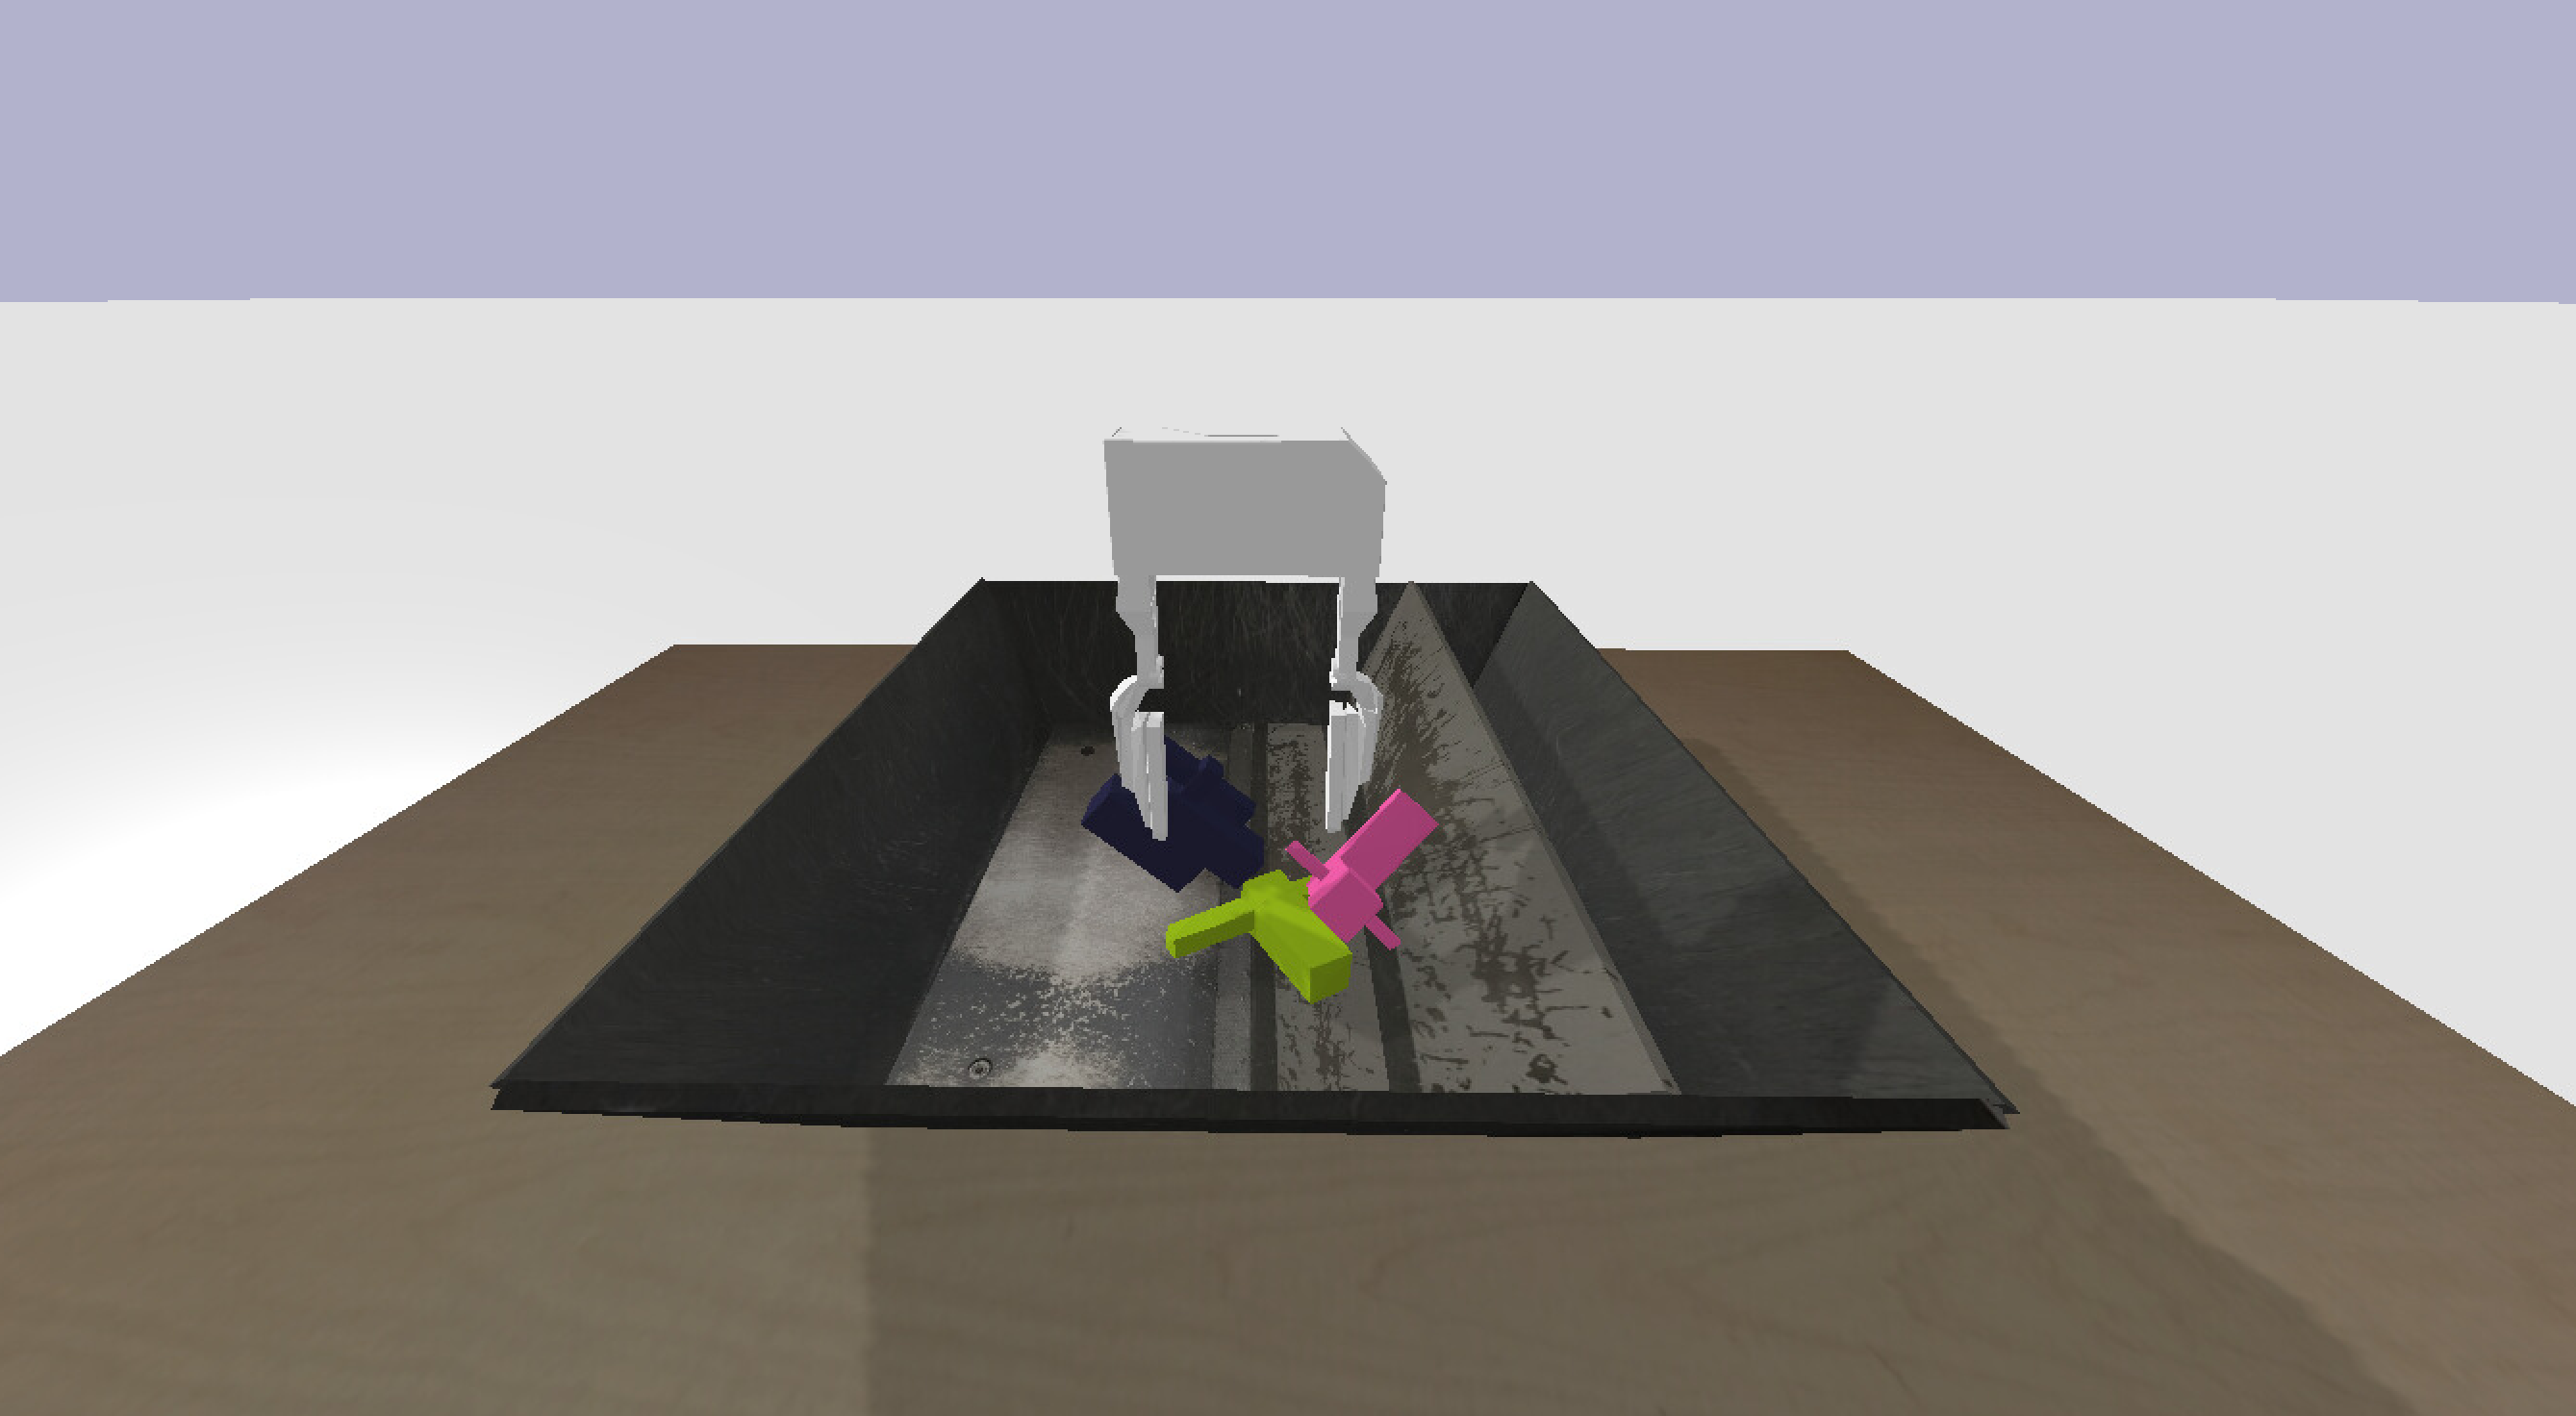
\includegraphics[width=\linewidth]{figures/tray.png}
      \caption{Table Scene} \label{fig:table}
    \end{subfigure}%
    \hspace*{\fill}   % maximize separation between the subfigures
    \begin{subfigure}{0.49\textwidth}
      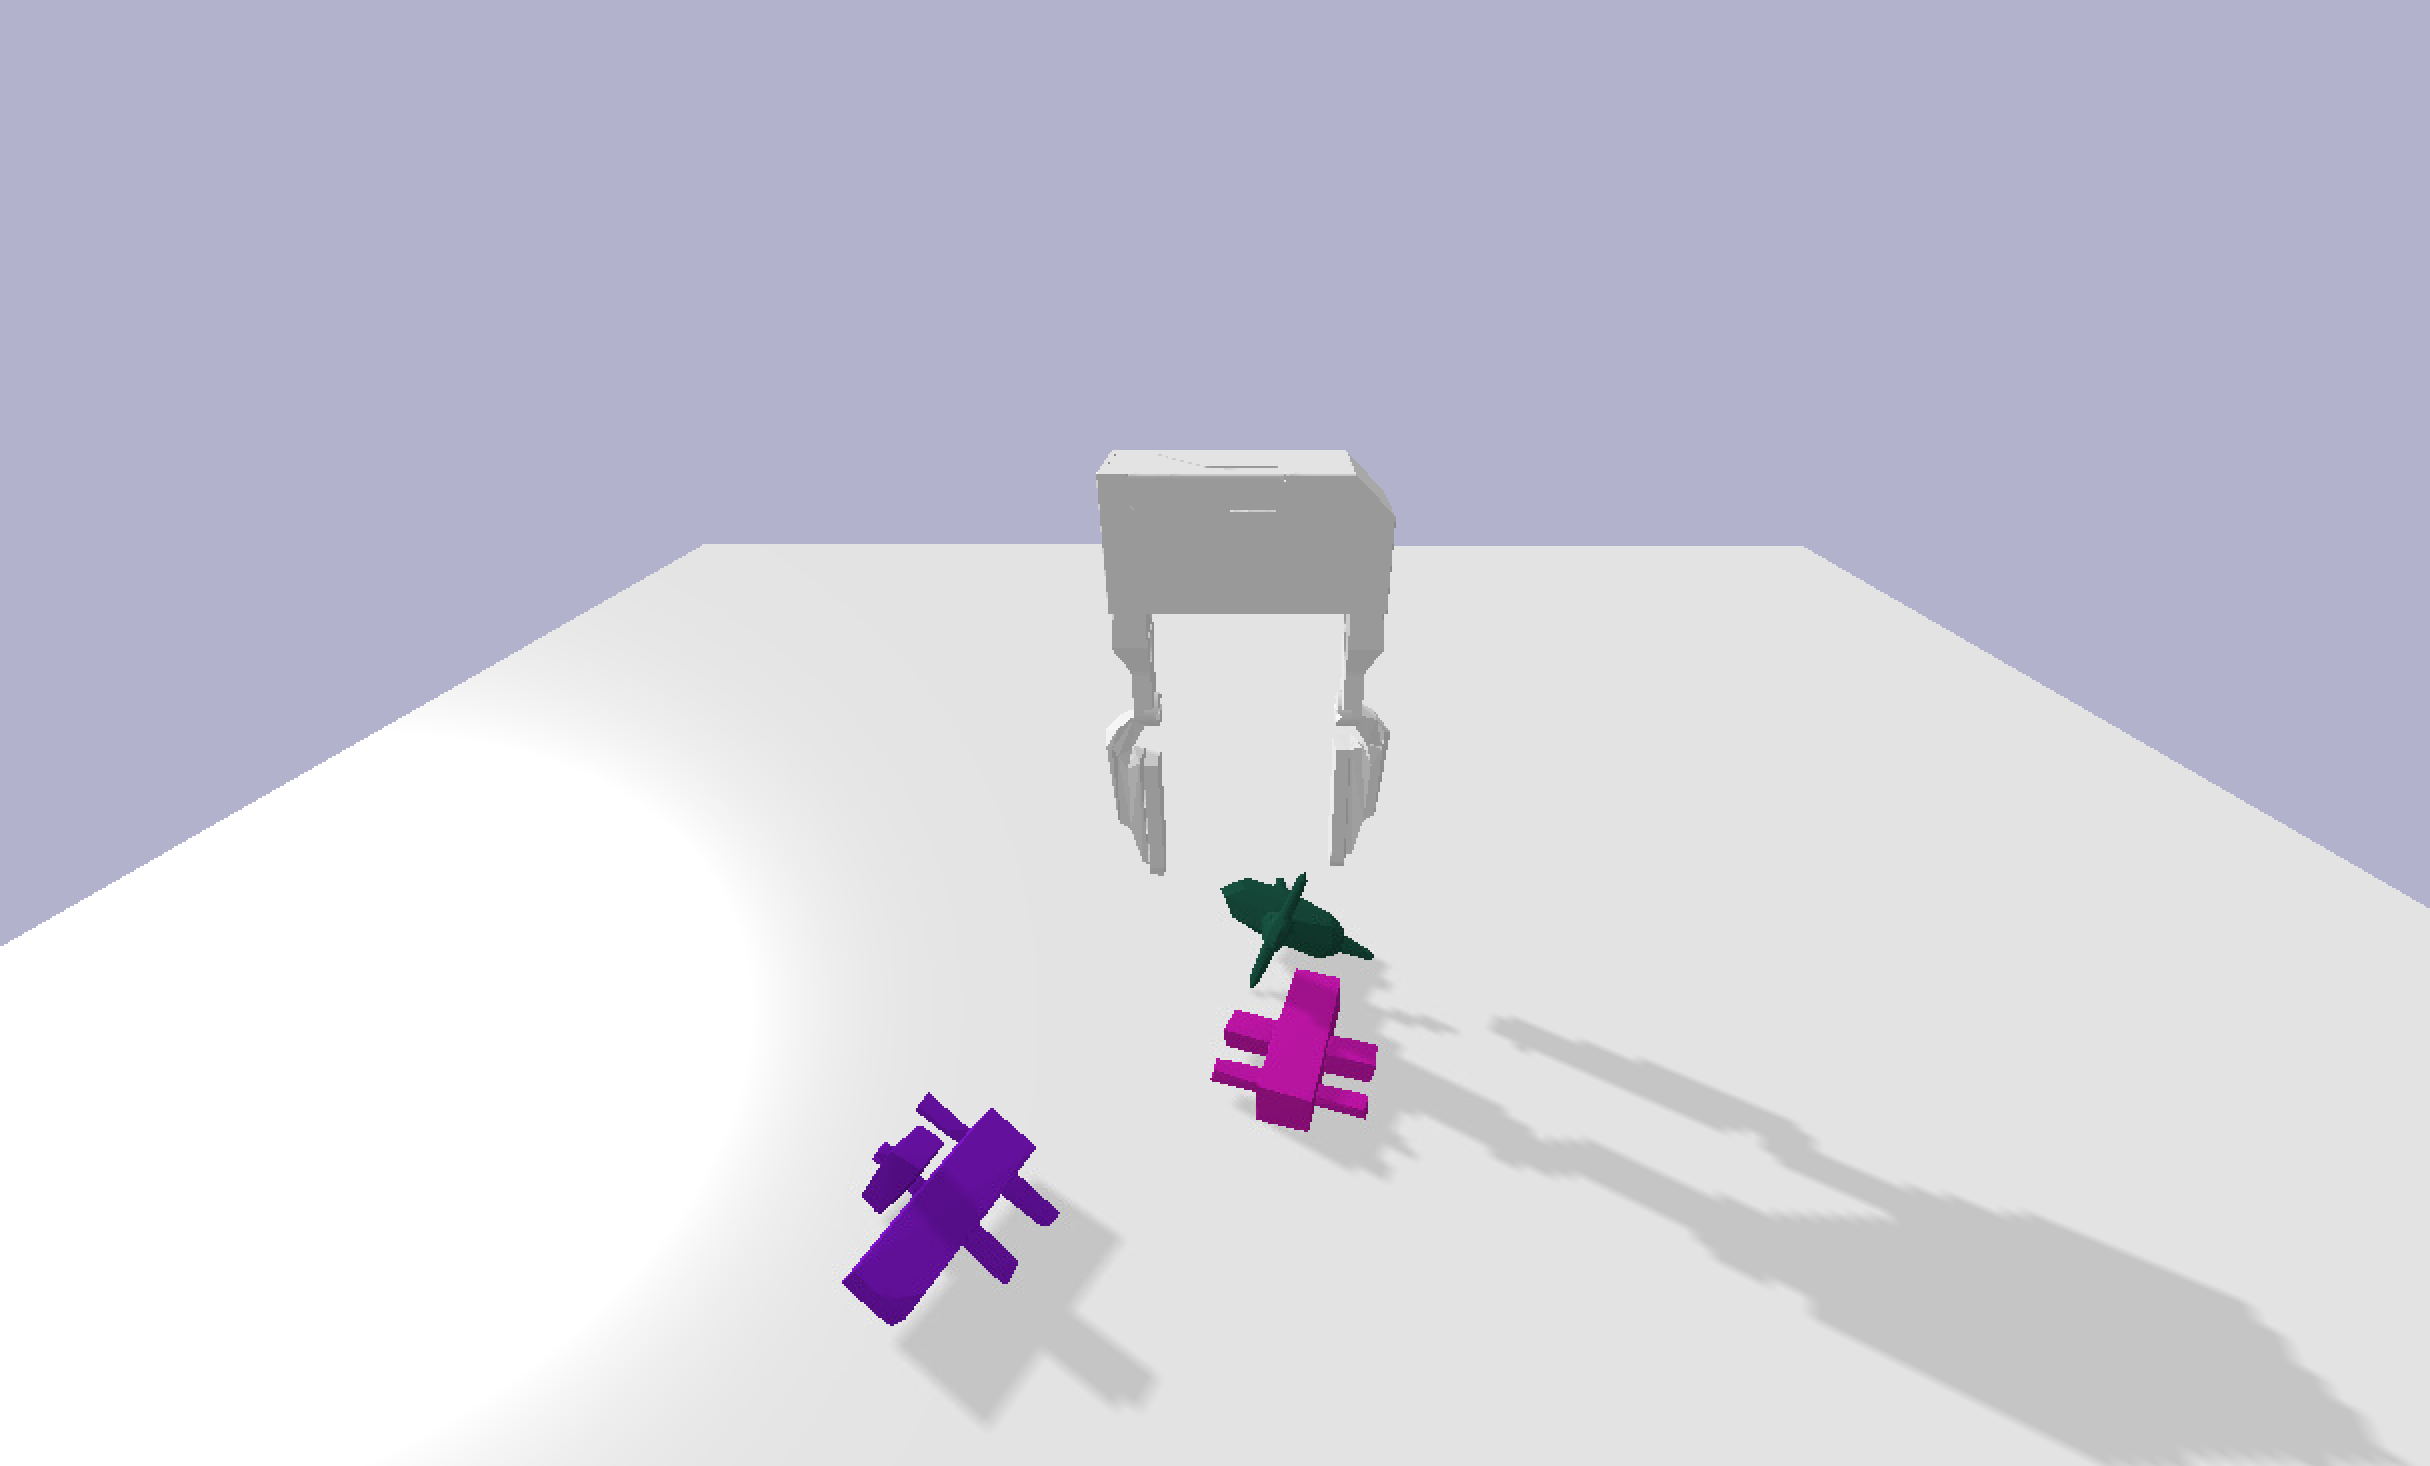
\includegraphics[width=\linewidth]{figures/floor.png}
      \caption{Floor Scene} \label{fig:floor}
    \end{subfigure}%
    \hspace*{\fill}   % maximize separation between the subfigures


\caption{ Table and floor scenes \label{fig:scenes}}
\end{figure}

\section{Robotics Environment Descriptions}

We have two testbed environments: one with the simplified task description, another is the full task description. We primarily use the simplified environment to test and prune the algorithms quickly. Only if the model solves the simplified environment, we move forward to try it in the full environment. Those two descriptions deviate in terms of action, observation, reward, and curriculum definition. 

The simplified environment has fewer action dimensions to control compare to the full environment. A total of three-dimensional action controls the x, y coordinates translation, and yaw rotation. Hence, every timestep it receives a fixed size of downward z-axis movement. Similar to Quillen et al. and Breyer et al. our gripper also automatically closes, when it reaches a certain height threshold

The full environment, on the other hand, has full control over all dimensions. In the full environment, the gripper receives five-dimensional action to control cartesian coordinates (x, y, z), yaw rotation, and the gripper open/close. 

Observation from the environment differs as well, based on the task description. In the simplified scenario agent only receives the hundred-dimensional encoded depth image. Whereas, in the full scenario, the agent gets the actuator width in addition to the hundred-dimensional encoder output. [\todo{yaz bir seyler daha} ]

We used a custom shaped reward function for the environment setting. In the simplified environment, a sparse reward definition was used. \todo{Better}

Curriculum strategy guides the agent to a more challenging environment structure based on the success rate of the agent. In our case, curriculum switch happens both on simplified and full environment definition at a \(70\%\) success rate. This switch triggers an increase of difficulty on the environment’s curriculum parameters such as max object count, object spawned area, and terminating object height.


\begin{figure}[htbp]
    \centering
    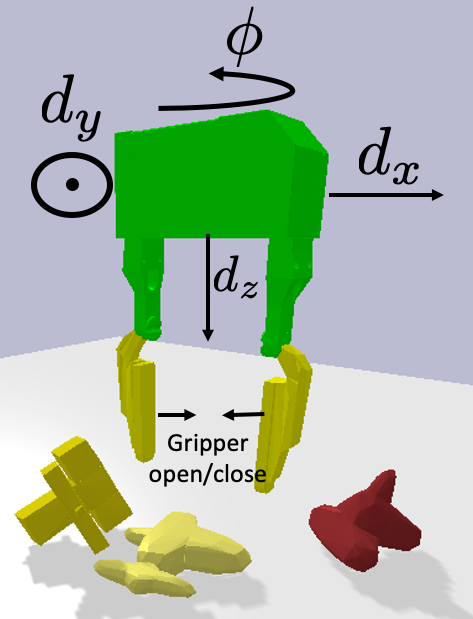
\includegraphics[width=0.3\linewidth]{figures/freedomDim.png}
\caption{Full environment freedom of movement} \label{fig:breyer}

\end{figure}


\begin{table}[htbp]
    \resizebox{\textwidth}{!}{
    \begin{tabular}{lllll}
    \toprule
     Env. Description     & Action Space & Observation                                           & Reward        & Discount Factor \\ \midrule % \hline
               Full       & 5            &  \shortstack{Encoder  + \\ Actuator Width or \\ RGBD \\ Depth} & Shaped Reward & 0.99  \\  \midrule % \hline
               Simplified & 3            & Encoder                                        & Binary Reward & 1.0    \\      %\hline
    \bottomrule
\end{tabular}}
\caption{Different paramters of Simplified and Full environment definitions}
\end{table}

\begin{table}[htbp]
    \resizebox{\textwidth}{!}{
    \begin{tabular}{llllll}
    \toprule
    Env. Description  & Curr Steps & Curr Success Thresh. & Robot Height & Max Objects & Object Area \\ \midrule
    Full                    & 8                & 0.7                          & [0.15, 0.25] & [3, 5]       & [0.01, 0.1]  \\ \midrule
    Simplified              & 4                & 0.7                          & [0.17, 0.27] & [3, 5]       & [0.01, 0.1]  \\ 
    \bottomrule
    \end{tabular}}
    \caption{Curriculum Parameters of Simplified and Full environment descriptions}
\end{table}


\section{Robot Model}
As mentioned in the problem setup section, we only use a gripper without the arm to increase computation speed. This setup obliviates the need for inverse kinematics calculation for each joint of a whole robotics arm. Although we deviate from the real-world setting by excluding the arm, Breyer et al. showed that the model learned without the entire kinematic chain can still perform successfully on the real-world robot \cite{Breyer2018}. This success is possible because of the small working setup comprising only 10cm to 10cm area and the limited translation and yaw rotation motions, 3cm and 15cm.

We noticed that in Breyer et al. setting, because of the narrow gripper width of the robot model (ABB Yumi), it could not perform at its maximum potential \ref{fig:breyer}. Thus, we selected a gripper (WSG50) that has a broader gripper opening \ref{fig:ourmodel}. As a result, we could use the object models without scaling.

\begin{figure}

    \begin{subfigure}{0.35\textwidth}
      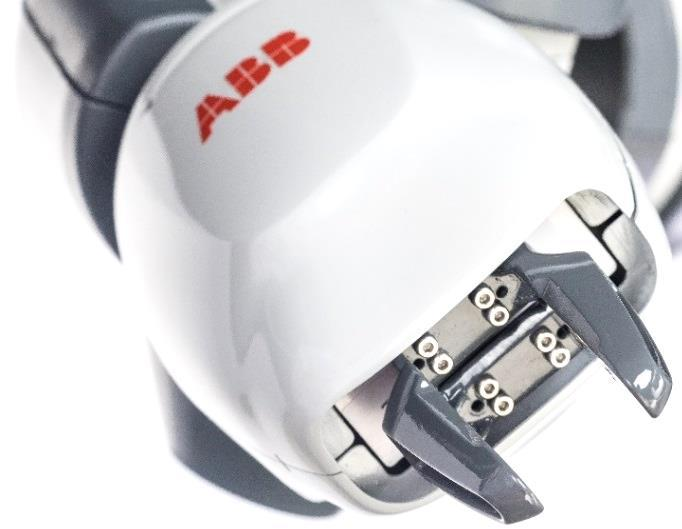
\includegraphics[width=\linewidth]{figures/abbyumi.jpg}
      \caption{ABB Yumi gripper model} \label{fig:ABBYUMI}
    \end{subfigure}%
    \hspace*{\fill}   % maximize separation between the subfigures
    \begin{subfigure}{0.35\textwidth}
      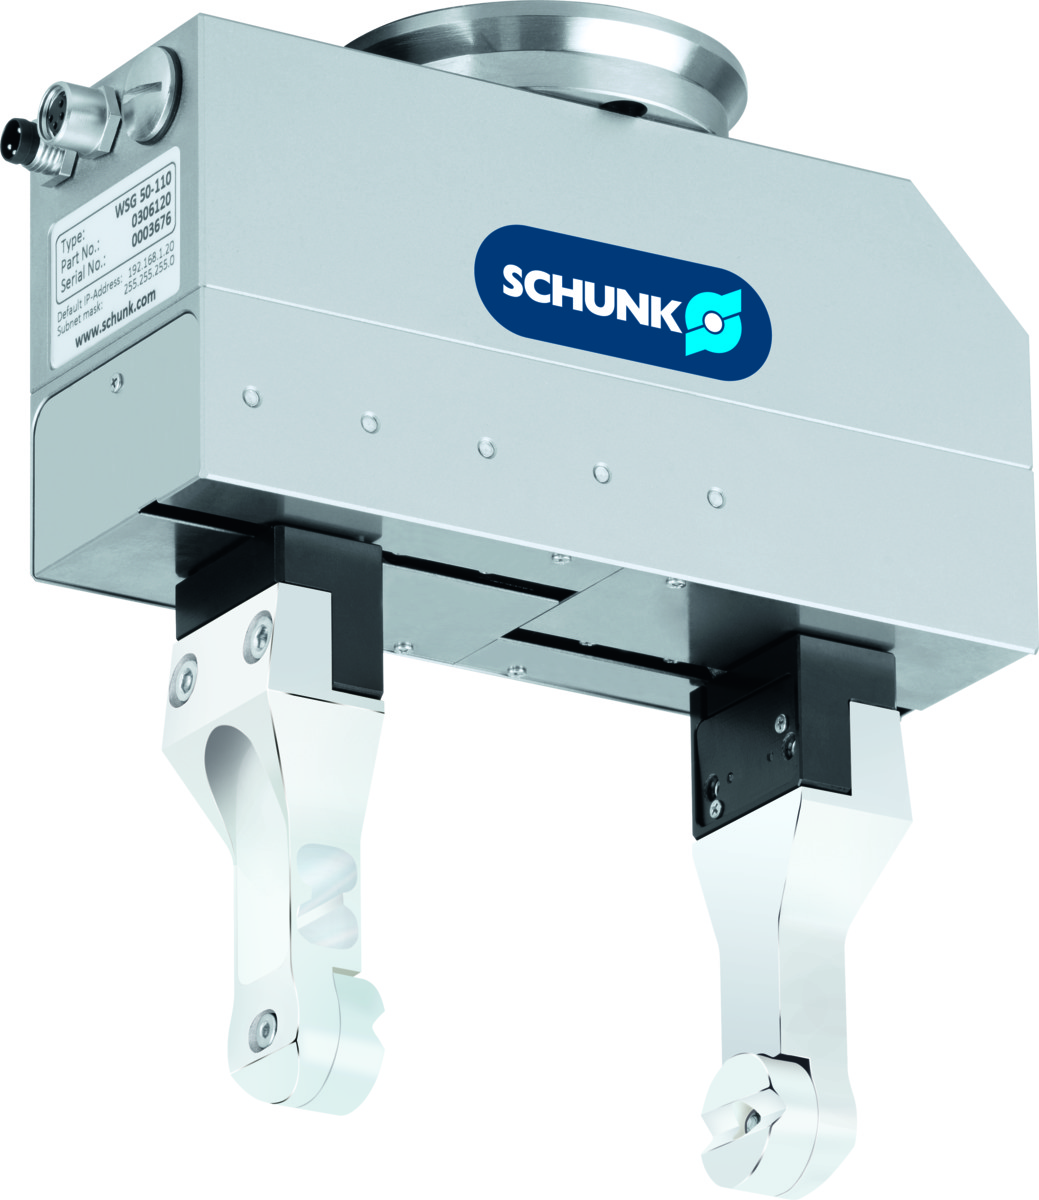
\includegraphics[width=\linewidth]{figures/wsg50.jpg}
      \caption{WSG50 gripper model} \label{fig:WSG50}
    \end{subfigure}%
    \hspace*{\fill}   % maximize separation between the subfigures


\caption{ Real images of gripper models   \label{fig:robots}}
\end{figure}

\begin{figure}

    \begin{subfigure}{0.49\textwidth}
      \includegraphics[width=\linewidth]{figures/breyerModel.png}
      \caption{ABB Yumi gripper used in Breyer et al.} \label{fig:breyer}
    \end{subfigure}%
    \hspace*{\fill}   % maximize separation between the subfigures
    \begin{subfigure}{0.49\textwidth}
      \includegraphics[width=\linewidth]{figures/ourModel.png}
      \caption{WSG50 gripper used in our work} \label{fig:ourmodel}
    \end{subfigure}%
    \hspace*{\fill}   % maximize separation between the subfigures


\caption{ Comparison of robot models \label{fig:robots}}
\end{figure}
\section{Object Database}

Generally, particular object shape and color usage bring a certain bias to the learned grasp model. Therefore, the object database should be as diverse as possible to encourage the model to perform well on novel objects. Indeed, the generalization of all different shapes and colors of the objects is our primary concern. Since we measure the success rate of an RL agent on the test set, a model that overfits the training dataset would perform poorly on the test set.

We use the random object database(\ref{fig:randomobj}) from pybullet-data \footnote{\url{https://bit.ly/3ijyCJM}} and the wooden-block datasets(\ref{fig:woodenobj}) from Breyer et al. for our experiments. We primarily trained on the random object database. Wooden blocks dataset was only used to test the robustness of the trained model.

Unlike, Quillen et al. and Breyer et al. which divided their dataset only into test and training, we used a validation set in addition to them.  We believe the inclusion of the validation set contributes to the generalization of the trained model. In total, test and validation sets have 150 objects each, and training sets consist of 700 objects.

\begin{figure}

    \begin{subfigure}{1.0\textwidth}
      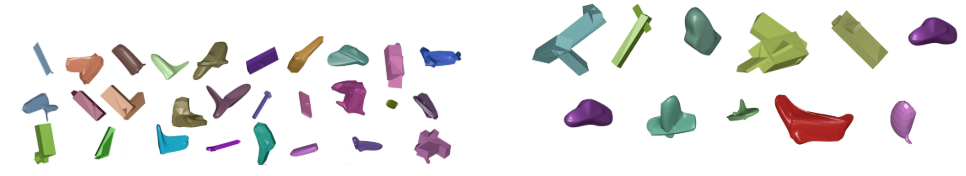
\includegraphics[width=\linewidth]{figures/random_objects}
      \caption{Random object dataset} \label{fig:randomobj}
    \end{subfigure}%
    \hspace*{\fill}   % maximize separation between the subfigures
    \newline
    \begin{subfigure}{1.0\textwidth}
      \centering
      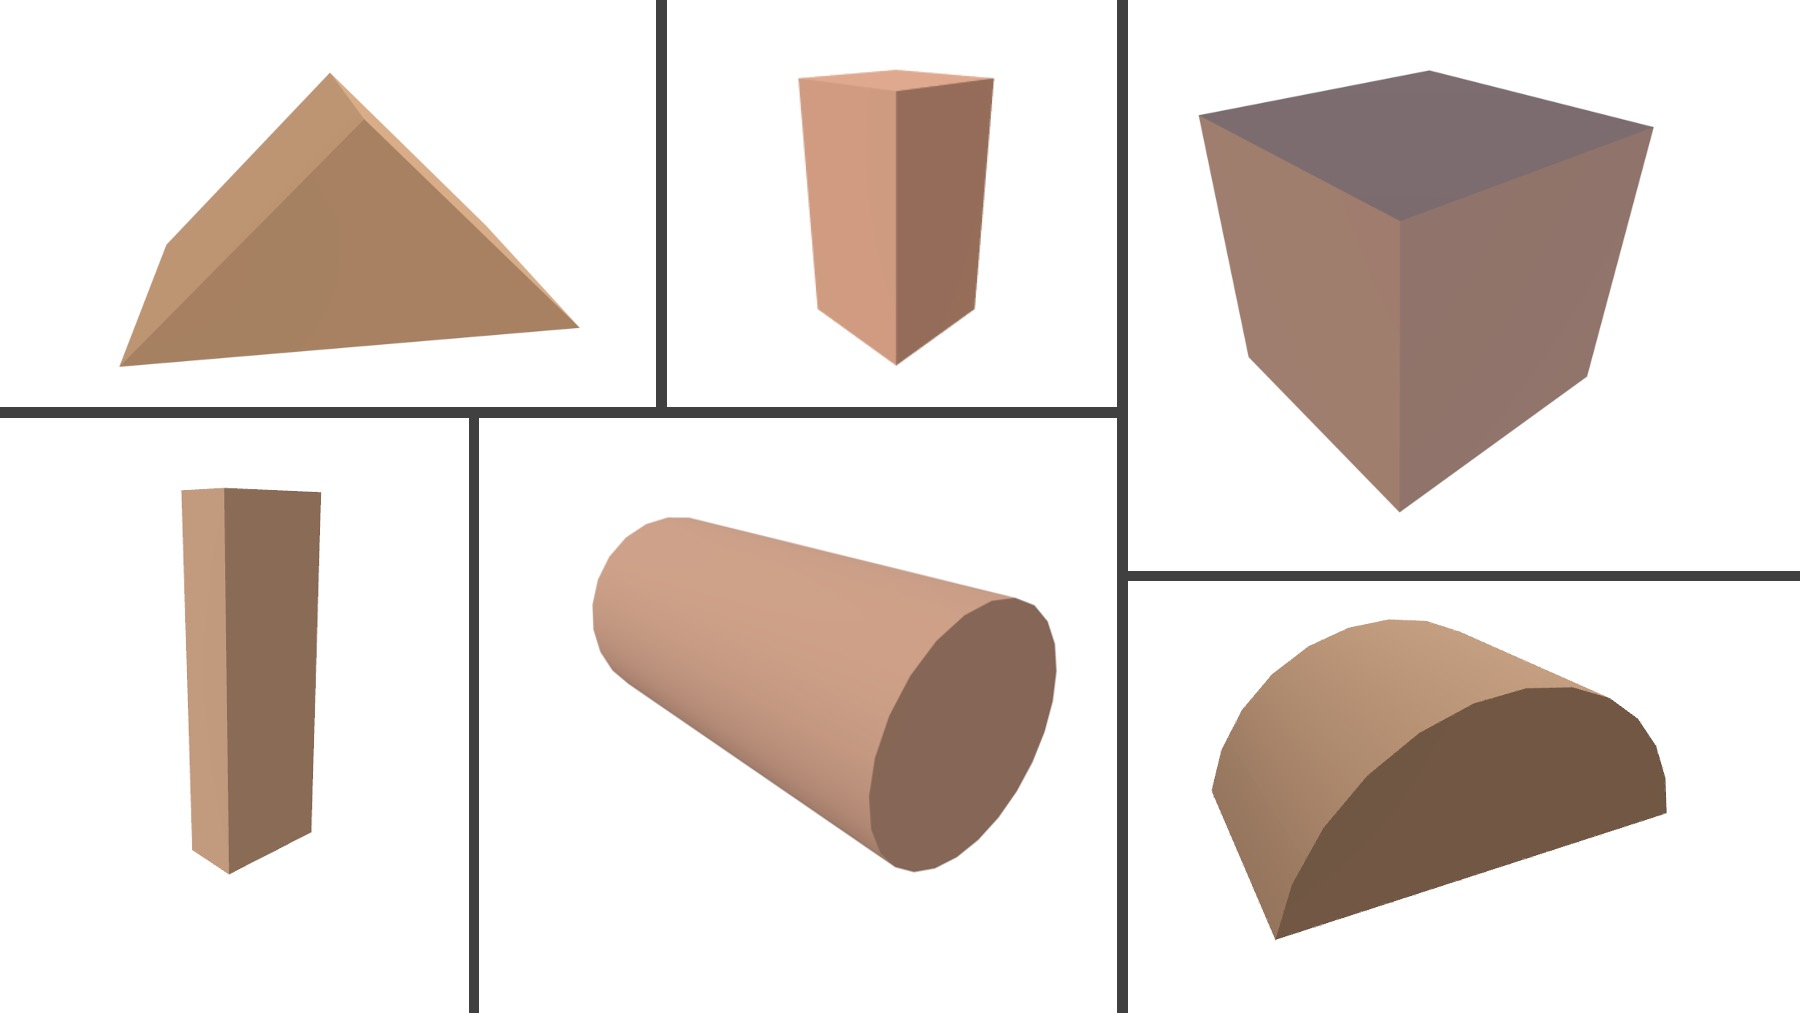
\includegraphics[width=0.3\linewidth]{figures/wooden_blocks}
      \caption{Wooden block dataset from Breyer et al. \cite{Breyer2018}} \label{fig:woodenobj}
    \end{subfigure}%
    \hspace*{\fill}   % maximize separation between the subfigures
\caption{ Different object datasets used in our work \label{fig:objdatasets}}
\end{figure}
\section{Data Acquisition}

We conduct all our experiments solely in the Bullet simulation engine. RL training needs an extreme amount of data and training time. The shortest training time required for our experiments is not shorter than a day. In this respect, simulation provides a low-cost, robust, and scalable stream of data \cite{openai2019rubiks}. Although low-quality sensor measurements pose a threat to simulation-based learning techniques, domain-randomization or continuous training strategies seem to mitigate the disadvantages of simulation. Akin to our work Breyer et al. trained a table cleaning gripper, which trained solely in simulation and performed a \(78\%\) success rate in the real robot \cite{Breyer2018}. In the contrast, Kalashnikov et al. collected all the robot training data in the span of four full months and 800 robot hours. They underlined the reality and quality of real-world collected data \cite{Kalashnikov2018}. 

The data acquisition process can be dealt with many different approaches. In our case, the most convenient choice was to lead the research entirely on simulation. We will explain more on the sim-to-real transfer and reality gap in the future work chapter.


\section{Observation}

The environment processes the observation data and serves it to the agent after each timestep. The observation here refers to the state of the agent in the Markov Decision Process \nameref{section:markov}. Observation consists of the encoded RGB-D sensor output similar to Breyer et al. We use the latent space of the auto-encoder to encode the large (64x64x3) RGB-D sensor output to (100x1). We collect 18000 training images and 2000 test images on a random agent working in the simplified environment description. We slightly change the data collection parameters of the Breyer et al. to allow closer images to the objects.

We also implemented a perception layer which allows the direct computation of RGBD sensor output. This approach makes use of a similar perception layer setup, as Mnih et al. We implemented two different types of non-encoded perception layers: RGBD sensor output with four separate channels and the depth sensor output with one channel. 

Processing of the raw sensor observations demands more delicate handling. Typically, we need to input the sensor output (RGBD or only Depth) to the convolutional neural network. However, the inclusion of the actuator width makes the processing more complicated. We ought to add the actuator width information to the sensor output without changing the sensor output's shape. In other words, we cannot flatten the sensor output and add the one-dimensional actuator width information. We need to pad the one-dimensional actuator width information into a three-dimensional array to comply with the sensor output (64x64x1 or 64x64x4). In the environment side, we truncate the padded actuator width information into the sensor output. Therefore, the actuator width information allocates a dedicated channel at the end of the whole environment observation. 

On the agent side, we parse the sensor output channels from the actuator width information again and input it to the observation processing neural network. This neural network consists of three convolutional neural layers and a fully connected layer at the end. After processing the sensor data, we get a one-dimensional array with 512 elements, which is the hidden layer size of the last fully connected layer. Then, we concatenate the unpadded actuator width information to the 512 elements fully connected layer output. In the end, we squeeze the observation into a one-dimensional array with 513 elements. This resulting array will be further processed in the agent's neural network that approximates either the Q-values, policy or both. Non-encoded observation process is explained with diagrams below \ref{fig:obsprocess}.

\begin{figure}[htbp]
    \centering
    \begin{subfigure}{1\textwidth}
      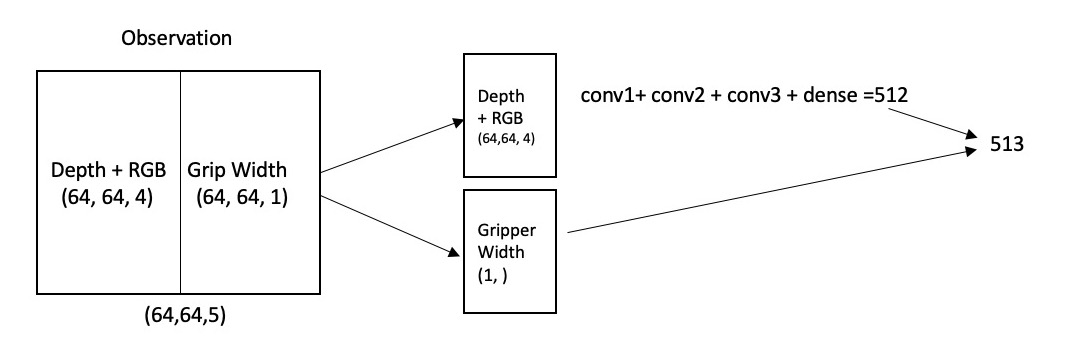
\includegraphics[width=1\linewidth]{figures/RGBDobs}
      \caption{RGBD output combined with gripper width. Overall shape (64,64,5)} \label{fig:rgbobs}
    \end{subfigure}%
    % \hspace*{\fill}   % maximize separation between the subfigures
    \newline
    \begin{subfigure}{1\textwidth}
      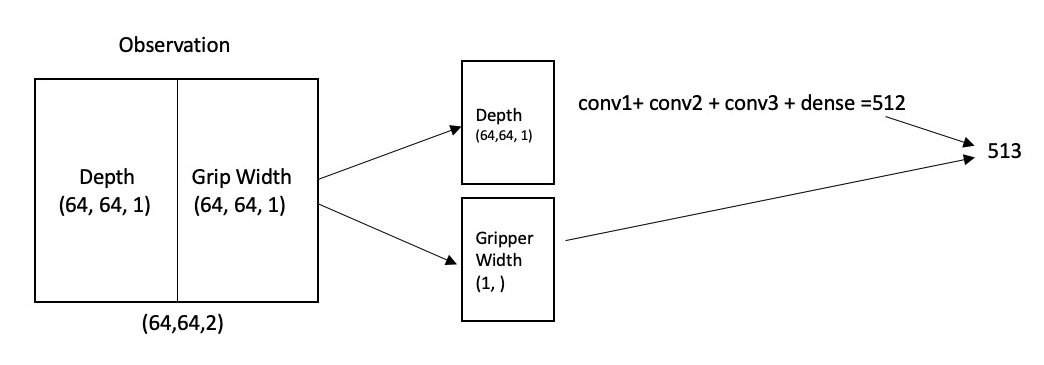
\includegraphics[width=1\linewidth]{figures/depthobs}
      \caption{Depth sensor output combined with gripper width. Overall shape (64,64,2)} \label{fig:depthobs}
    \end{subfigure}%
    % \hspace*{\fill}   % maximize separation between the subfigures


\caption{ Non-encoded observation processing layers \label{fig:obsprocess}}
\end{figure}
\section{Reward Structure}

As mentioned in the environment description section, we use different reward definitions for simplified and full environments. Simplified environment definition uses sparse reward, meaning when success, the agent receives 1 otherwise 0. The full environment definition handles the learning with a more sophisticated shaped reward function. 
Shaped reward function awards both the terminal state and sub-goals such as grasping and lifting the object, whereas it penalizes every spent time before the terminal state. Rewards and time penalty are defined below.

\begin{align*}
    \text{Terminal Reward: } r_t = 10000 \\
    \text{Grasping Reward: } r_g = 100 \\
    \text{\(\Delta\)h Scale Coefficient: } c = 1000 \\
    \text{Time Penalty: } r_{tp} = 200
\end{align*}


The shape reward function guides the robot to the terminal state by defining sub-goals. Otherwise, the agent may need to spend way too much time to explore the terminal state. In other words, rewards function sets up curriculum-like learning objectives to facilitate the learning. The reward function is given in equation \ref{eq:reward_eqn}. 

\begin{equation}
    r = (\text{grasp detected}).(r_g + c. \Delta h) - r_{tp}
    \label{eq:reward_eqn}    
\end{equation}


One needs to pay attention that each state except the terminal state, the step reward should be negative. This condition guarantees the maximum reward the agent receives is linked to reaching the terminal state as soon as possible. If a step reward is positive, the agent will try to stay at that state as long as it can to increase its reward, before going to the terminal. Thus, it contradicts our training goal: the best performing agent collects the objects as soon as possible. The timestep penalty should always be greater than the sum of grasp reward and lifting rewards to avoid the contradictory reward situation. This condition is formalized with the given inequality. Note that the time penalty is a positive number.

\begin{equation}
 r_{tp} > r_g + c \Delta h
\end{equation}

\begin{equation}
    \text{Shaped Reward:}
    \begin{cases}
    \text{Grasp}: \begin{cases} \text{Non-Terminal} : r_g + c.\Delta h -r_{tp} \\ 	
                                \text{Terminal} : r_t - r_{tp}
    \end{cases} \\
    \text{No Grasp}: \begin{cases} \text{Non-Terminal} : -r_{tp}\\ 
                                    \text{Terminal}= \text{Timeout}: -r_{tp} 
    \end{cases}
    \end{cases}
\end{equation}
\section{Actions}

There are two parts to the action definition. One part defines an interface with OpenAI Gym to let interact with the agent. The other part is the environment, receiving the action and processing it further, such as cropping it and scaling it. An example of an action space definition is given below \ref{code:actdefine}. 

\begin{lstlisting}[language=Python, caption=OpenAI gym action space definition, label=code:actdefine]

    if not self._discrete:
        self.action_space = gym.spaces.Box(-1.,
                                             1., shape=(3,), dtype=np.float32)
    else:
        self.action_space = gym.spaces.Discrete(self.num_actions_pad*3)

\end{lstlisting}


It defines the action type and the shape of the action. This definition is later processed by the RL algorithm to output an action based on what the environment expects. Our environment takes only continuous actions. However, we linearly discretized the environment to comply with the DQN algorithm's discrete action space. Based on the discretization padding given in the configuration file, we define the size of the discrete action space. For instance, if the discretization padding is three for each action dimension, and if the simplified environment is set, we would have nine actions. Since the simplified environment has three actions dimension and three actions padding for each action makes up in a total of nine actions. The below diagram presents the linear action discretization \ref{fig:disc}.

\begin{figure}[htbp]
    \centering
    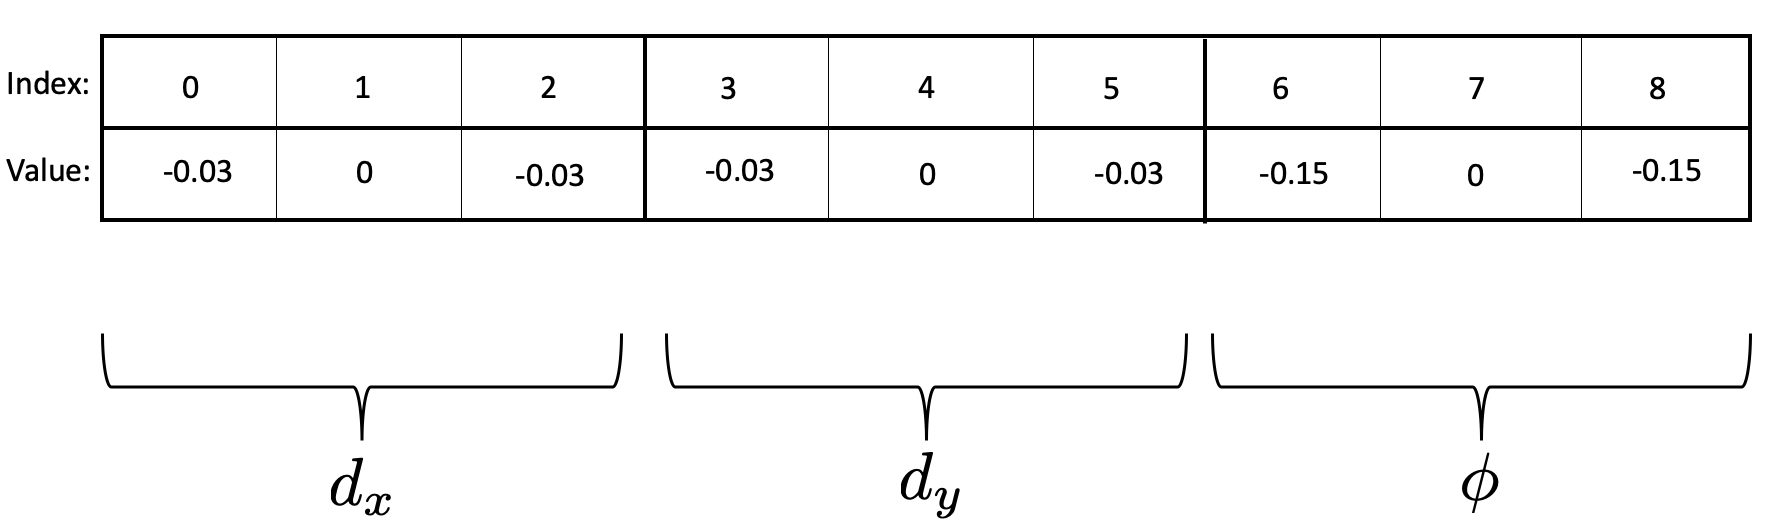
\includegraphics[width=1\textwidth]{figures/discretization.png}
    \caption{Linear action discretization representation. Padding one action dimenstion is 3 and total number of action dimension is 3}
    \label{fig:disc}
\end{figure}

As mentioned in Stable-Baselines documentation \footnote{\url{https://bit.ly/2PYe5hG}} continuous actions algorithms work best when the action space is defined symmetric and between -1 and 1. Therefore, we need to rescale the actions in the environment side to fit the maximum action limits. This problem does not appear in the discrete action space because we already receive the action index from the DQN algorithm and can easily assign it to the respective values.
\section{Training Structure}

As described in the hardware setup section, we train on LRZ compute cloud mainly. Given that we cannot monitor the status of training always, we obliged to implement a robust training structure to overcome the unexpected death of the processes[\todo{better}]. Also, in general, machine learning by nature is not always improving throughout the training process. The model performance might well get worse towards the end of the training. One way to avoid this problem is to implement checkpoint and evaluation callbacks to inspect the model performance at regular intervals. Another way to achieve robust training is to monitor the training process and log the results to a CSV file. This way, we can overview the training process and judge where to end the training. We primarily monitor the training loss, success rate, and reward.

With the help of evaluation callback, we validate the model performance on a different instance of the gripper environment with the validation object set. We regularly save the best performing model based on average reward over ten episodes. This process assures that we will always have the best-generalized model. If the training unexpectedly ends or the loss increases, we would have a model to judge the performance. We repeat the training process evaluation every 50000 timesteps. Besides, we save the agent model every 25000 timesteps to assure a minimum loss in case of a sudden stop of the training process.
The monitoring procedure is taken care of by the modified version of Stable Baselines monitor wrapper.  We extended the wrapper class\footnote{\url{https://bit.ly/2CtoEX1}} to save the timestep, success rate, and curriculum lambda in addition to reward and episode information.


\begin{lstlisting}[language=Python, caption= Integration of monitor wrapper helper function, label=code:monitor]


    Monitor(gym.make('gripper-env-v0', config=config), "log_file")


\end{lstlisting}

Moreover, we implemented a parameterized training structure to allow users to try different configurations quickly. We parameterized input and reward normalization and time-feature wrapper.

% \section{Testing Structure}
    % \subsection{Run the Code}
% \section{Curriculum Integration}
    % \subsection{Curriculum Parameters}
% \section{Hyperparameter Search}
% \section{GPU vs. CPU}
